\documentclass[tikz,border=6pt]{standalone}
\usepackage[utf8]{inputenc}
\usepackage[T1]{fontenc}
\usepackage{amsmath,amssymb}
\usepackage{lmodern}
\usetikzlibrary{arrows.meta}

\definecolor{ink}{HTML}{1d1d1f}
\definecolor{sub}{HTML}{515154}
\definecolor{muted}{HTML}{6e6e73}
\definecolor{amber}{HTML}{c76008}
\definecolor{amberbright}{HTML}{ff9f0a}
\definecolor{amberfill}{HTML}{fff3e0}
\definecolor{blue}{HTML}{0066cc}
\definecolor{bluefill}{HTML}{e8f2ff}
\definecolor{redbright}{HTML}{ff453a}

\begin{document}
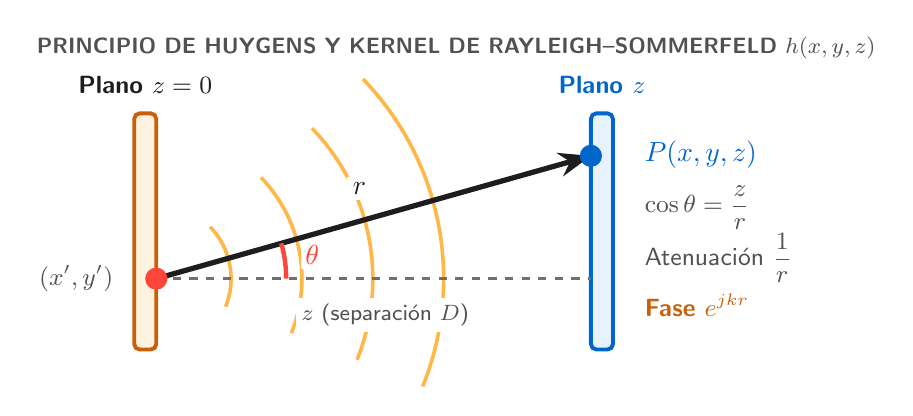
\begin{tikzpicture}[font=\sffamily,>=Stealth]

\node[anchor=west,font=\sffamily\bfseries\footnotesize,text=sub] at (0,4.55)
  {PRINCIPIO DE HUYGENS Y KERNEL DE RAYLEIGH--SOMMERFELD $h(x,y,z)$};

% Plano z = 0
\node[font=\sffamily\small\bfseries,text=ink] at (1.50,4.08) {Plano $z = 0$};
\filldraw[fill=amberfill,draw=amber,line width=1.4pt,rounded corners=2pt]
  (1.36,0.72) rectangle (1.64,3.72);

% Plano z
\node[font=\sffamily\small\bfseries,text=blue] at (7.30,4.08) {Plano $z$};
\filldraw[fill=bluefill,draw=blue,line width=1.4pt,rounded corners=2pt]
  (7.16,0.72) rectangle (7.44,3.72);

% Arcos esféricos de Huygens desde (x',y',0)
\coordinate (src) at (1.64,1.62);
\foreach \rad in {0.95, 1.85, 2.75, 3.65} {
  \draw[amberbright,line width=1.3pt,opacity=0.75]
    (src) ++(-22:\rad) arc (-22:44:\rad);
}

% Eje horizontal z
\draw[muted,dashed,line width=1.2pt] (src) -- (7.16,1.62);
\node[fill=white,inner sep=2pt,font=\sffamily\footnotesize,text=sub] at (4.55,1.16)
  {$z$ (separación $D$)};

% Vector r hacia P(x,y,z)
\coordinate (dst) at (7.16,3.18);
\draw[->,ink,line width=1.9pt] (src) -- (dst);
\node[fill=white,inner sep=2pt,font=\sffamily\normalsize\bfseries,text=ink] at (4.22,2.76) {$r$};

% Ángulo theta
\draw[redbright,line width=1.6pt] (src) ++(0:1.65) arc (0:15.8:1.65);
\node[fill=white,inner sep=1.5pt,font=\sffamily\normalsize\bfseries,text=redbright] at (3.62,1.92) {$\theta$};

% Puntos emisor y receptor
\fill[redbright] (src) circle (4pt);
\node[anchor=east,font=\sffamily\small\bfseries,text=sub] at (1.22,1.62) {$(x',y')$};

\fill[blue] (dst) circle (4pt);

% Anotaciones a la derecha
\node[anchor=west,font=\sffamily\normalsize\bfseries,text=blue] at (7.72,3.20) {$P(x,y,z)$};
\node[anchor=west,font=\sffamily\small,text=sub] at (7.72,2.52) {$\cos\theta = \dfrac{z}{r}$};
\node[anchor=west,font=\sffamily\small,text=sub] at (7.72,1.88) {Atenuación $\dfrac{1}{r}$};
\node[anchor=west,font=\sffamily\small\bfseries,text=amber] at (7.72,1.28) {Fase $e^{jkr}$};

\end{tikzpicture}
\end{document}
